\section{Pre-study}
	\subsection{Solution today}
		\subsubsection{Existing functionality}
Since the application already is considered a working prototype, we will provide a list which gives a description for the functionality. Working functionality is in this report defined as the functionality that is implemented in the frontend or backend. If something is implemented backend it has to be used frontend. A more detailed techincal description is found in the architecture-section.

\begin{figure}[h!]
\begin{center}
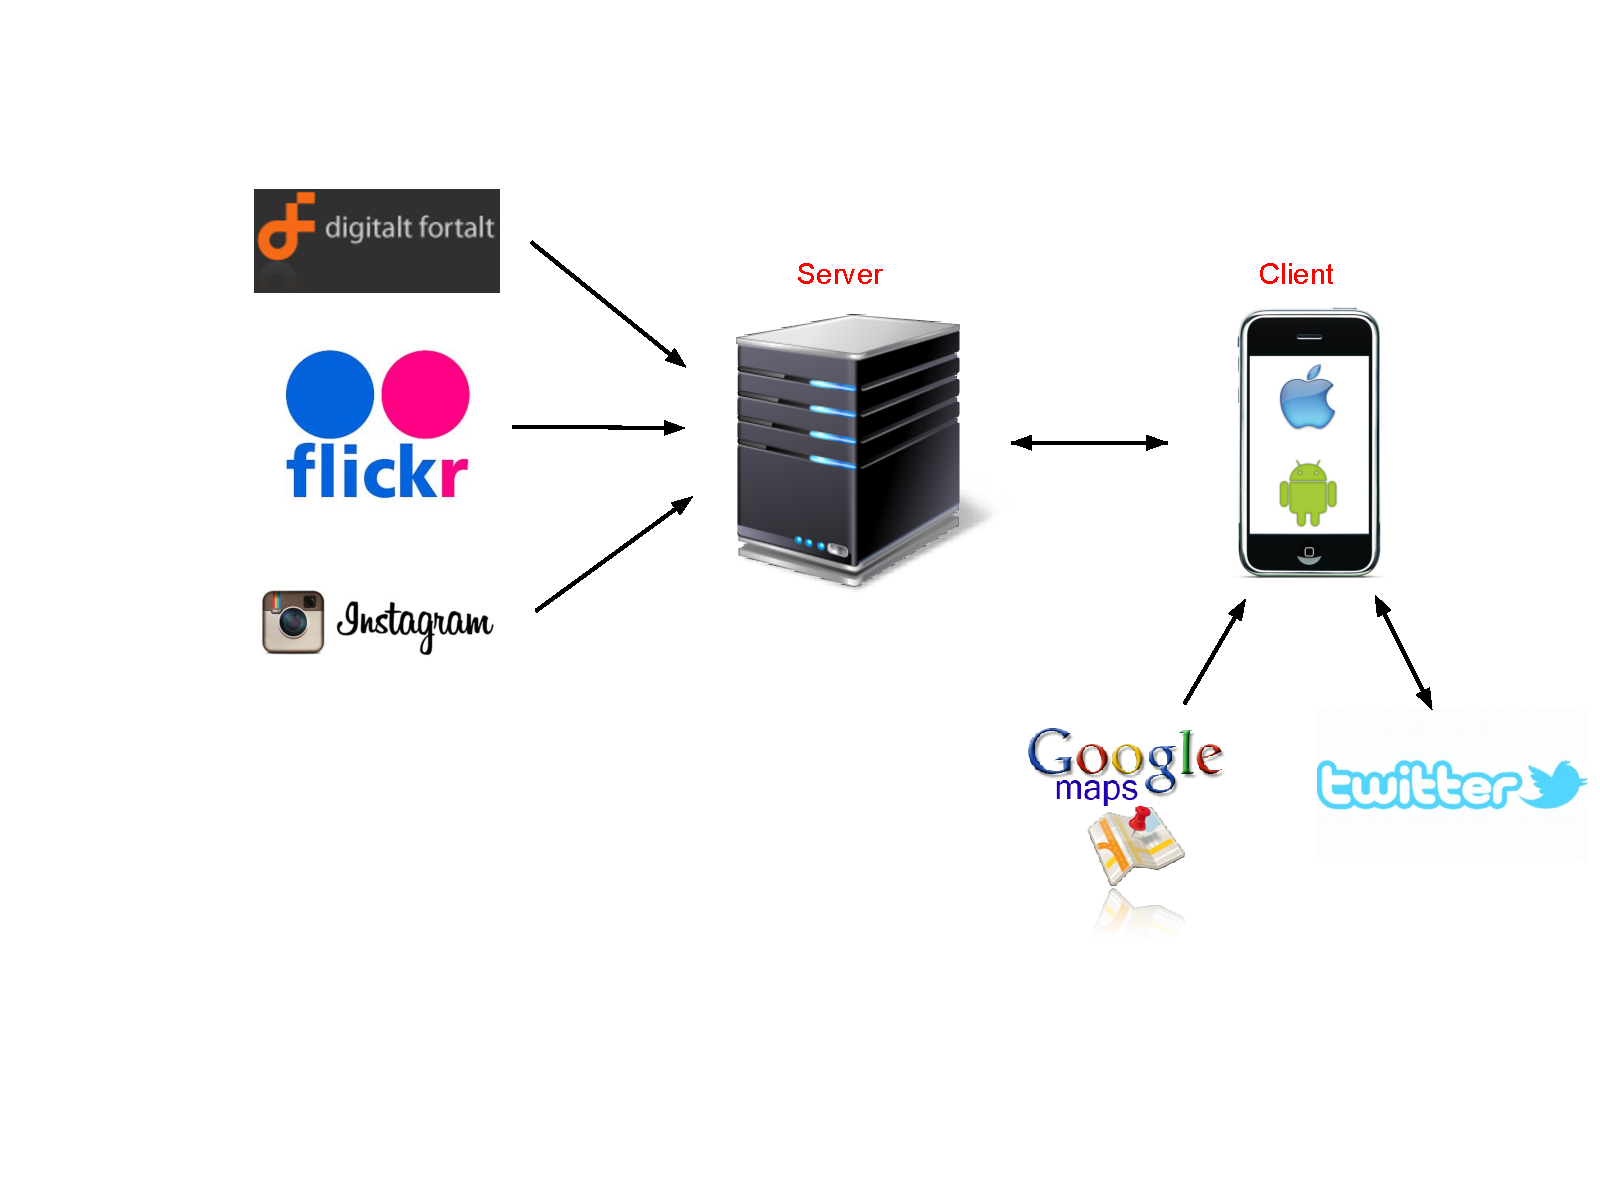
\includegraphics[scale=0.45]{ntoverview-architecture}
\caption{A simple overview of the architecture}
\end{center}
\end{figure}

\begin{itemize}
\item Browse a map and zoom in and out.
\item Load \textbf{places}.
\item Click on a place in the map and access \textbf{stories} from Digitalt Fortalt.
\item Get social media related to a place from the content providers Instagram and Twitter.
\item Go to a users exact position on a map.
\item Search for a location in the map.
\end{itemize}
	
		\subsubsection{Limitations}
There are some limitations to the system that needs to be further developed, and some that probably would require total architectural review of the project to be fixed. Our task is to continue the development of the applicaton. An overview of the features we are going to improve are discussed in the requirements-section. Flaws that arised during the development which requires a new architecture will be discussed in the conclusions-section under Recommendations.

		\subsubsection{Evaluation}
		
		\todo{Oversette sammendrag av vår samlede evaluering av appen}
		
	\subsection{Survey}

	\todo{Sammendrag av spørreundersøkelsen som ble gjort av Øyvind}
	
	\subsection{Desired solution}
	
	\todo{Implementere requirements i en liten tekst som forklarer hva vi ønsket å oppnå med applikasjonen}
	
	\subsection{Tools and technologies}
		\subsubsection{Titanium vs Phonegap}
		\subsubsection{Digitalt fortalt API}
	
	\subsection{Similar products}
		\todo{produkter med ligjnende funksjonalitet og/eller produkter med liknende formål}
